\documentclass{beamer} 
\usepackage{tikz}
\usepackage[all]{xy}
\usepackage{amsmath,amssymb}
\usepackage{hyperref}
\usepackage{graphicx}
\usepackage{algorithmic}
\usepackage{multirow}

\DeclareMathOperator*{\argmin}{arg\,min}
\DeclareMathOperator*{\Lik}{Lik}
\DeclareMathOperator*{\PoissonLoss}{PoissonLoss}
\DeclareMathOperator*{\Peaks}{Peaks}
\DeclareMathOperator*{\Segments}{Segments}
\DeclareMathOperator*{\argmax}{arg\,max}
\DeclareMathOperator*{\maximize}{maximize}
\DeclareMathOperator*{\minimize}{minimize}
\newcommand{\sign}{\operatorname{sign}}
\newcommand{\RR}{\mathbb R}
\newcommand{\ZZ}{\mathbb Z}
\newcommand{\NN}{\mathbb N}
\newcommand{\z}{$z = 2, 4, 3, 5, 1$} 

\newcommand{\algo}[1]{\textcolor{#1}{#1}}
\definecolor{PDPA}{HTML}{66C2A5}
\definecolor{CDPA}{HTML}{FC8D62}
\definecolor{GPDPA}{HTML}{4D4D4D}

% Set transparency of non-highlighted sections in the table of
% contents slide.
\setbeamertemplate{section in toc shaded}[default][100]
\AtBeginSection[]
{
  \setbeamercolor{section in toc}{fg=red} 
  \setbeamercolor{section in toc shaded}{fg=black} 
  \begin{frame}
    \tableofcontents[currentsection]
  \end{frame}
}

\begin{document}

\title{Interpretable machine learning algorithms for understanding factors related to childhood autism}

\author{
  Toby Dylan Hocking\\
  toby.hocking@nau.edu\\
  toby.hocking@r-project.org\\
}

\maketitle

\begin{frame}
  \frametitle{Motivation and data for predicting childhood autism}
  \begin{itemize}
  \item We have data from the National Survey of Children's Health.
  \item Each year a number of people fill out the survey (rows), and
    we have data for their responses (columns).
%download-nsch-data/nsch_2018_topical.do:292:label var k2q35a  "Autism ASD"
  \item One column, k2q35a ``Autism ASD'' (Yes or No) represents if
    the child has Autism.
  \item \textbf{Data pre-processing}: operations prior to machine
    learning.
  \item \textbf{Prediction accuracy in a given year}: can we predict
    Autism variable (output/label/dependent), given the others?
    (inputs/features/independent)
  \item \textbf{Model interpretation / feature selection}: which
    inputs are most useful for prediction?
  \item \textbf{Similarity/difference between years}: Can we train
    on one survey year, and accurately predict on another?
  \end{itemize}
\end{frame}

\section{Data pre-processing}

\begin{frame}
  \frametitle{Data pre-processing}

  \begin{itemize}
  \item Download NSCH data from public Census web site.
  \item For each year, keep all columns with less than
    10\% missing values, then remove all rows with at least one missing value.
  \item One-hot recoding of categorical variables (create 0/1
    dummy/indicator variable for each value).
  \item Then keep only columns in common between both years: result is
    46,010 rows and 366 columns. Details:
  \end{itemize}

  \scriptsize
  
  % latex table generated in R 4.3.2 by xtable 1.8-4 package
% Sun Feb 25 15:33:26 2024
\begin{tabular}{rlrrrrrr}
  \hline
year & data.type & nrow & ncol & questions & \%Autism & \%rowsNA & \%colsNA \\ 
  \hline
 2019 & raw & 29433 &   443 &   443 & 2.9615 & 100.0000 & 90.0677 \\ 
   2019 & processed & 18202 &   377 &   187 & 2.9997 & 0.0000 & 0.0000 \\ 
   2020 & raw & 42777 &   443 &   443 & 2.9758 & 100.0000 & 90.0677 \\ 
   2020 & processed & 27808 &   373 &   185 & 3.0818 & 0.0000 & 0.0000 \\ 
   \hline
\end{tabular}
 

Data source:

\url{http://www2.census.gov/programs-surveys/nsch/datasets/2019/nsch_2019_topical_Stata.zip} nsch\_2019\_topical.dta, nsch\_2019\_topical.do

\url{http://www2.census.gov/programs-surveys/nsch/datasets/2020/nsch_2020_topical_Stata.zip} nsch\_2020\_topical.dta, nsch\_2020\_topical.do

\end{frame} 

\begin{frame}[fragile]
  \frametitle{One-hot encoding of categorical variables}

Sometimes called dummy/indicator variables in statistics. 

For each value, we create a new column with 0/1 values.

For example, from \verb|nsch_2020_topical.do|
\begin{verbatim}
label var k4q24_r  "Specialist Visit"
label define k4q24_r_lab  1  "Yes"
label define k4q24_r_lab  2  "No, but this child needed 
 to see a specialist", add
label define k4q24_r_lab  3  "No, this child did not 
 need to see a specialist", add
\end{verbatim}
code above means there is a column named \verb|k4q24_r| in \verb|nsch_2020_topical.dta|, with values 1, 2, 3.

In our analysis we use a one-hot encoding, which means deleting that
column, and creating two 0/1 columns:

\small
\verb|Specialist Visit=Yes| and
\verb|Specialist Visit=No, but this child needed to see a specialist|

\end{frame}

\section{Prediction accuracy in a given year}

\begin{frame}
  \frametitle{K-fold cross-validation: a standard algorithm used to estimate the prediction accuracy in machine learning}
  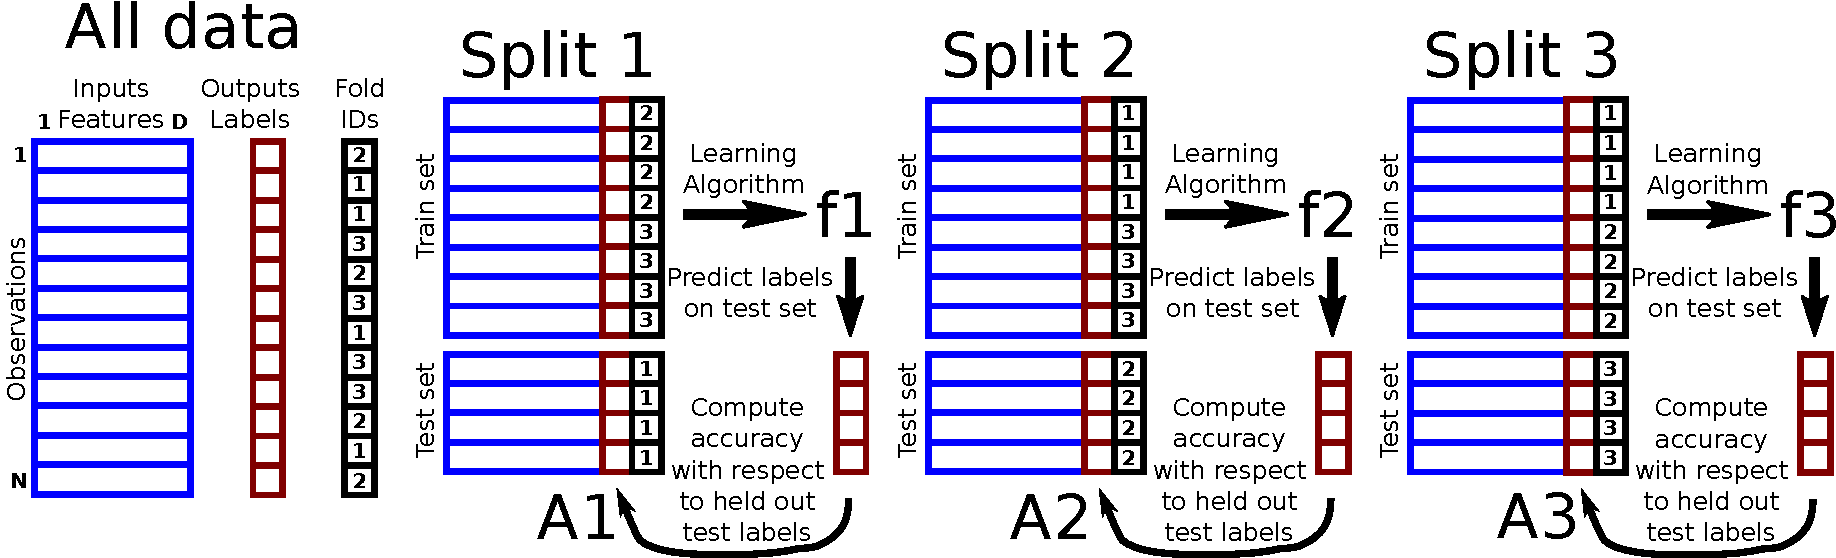
\includegraphics[width=\textwidth]{drawing-cross-validation.pdf}
\end{frame}

\begin{frame}
  \frametitle{10-fold cross-validation for comparing learning algorithms}
  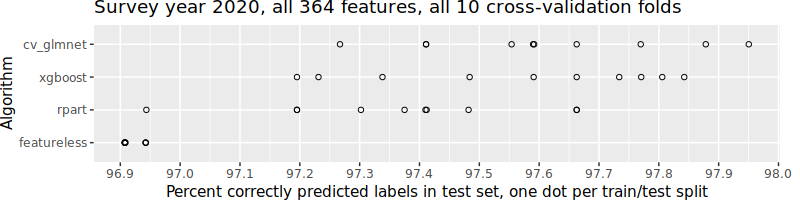
\includegraphics[width=\textwidth]{download-nsch-mlr3batchmark-registry-one-set-all-features.png}
\end{frame}

\begin{frame}
  \frametitle{Summarize 10 folds with mean and standard deviation}
  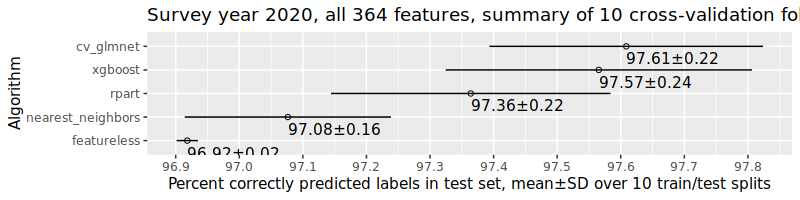
\includegraphics[width=\textwidth]{download-nsch-mlr3batchmark-registry-one-set-all-features-stats.png}
\end{frame}

\begin{frame}
  \frametitle{Confusion matrix and error rates}
  \begin{tabular}{c|c|c}
    & Label 0            & Label 1 \\
    \hline
    Predict 0 & True Negative (TN) & False Negative (FN) \\
    \hline
    Predict 1 & False Positive (FP)& True Positive (TP)
  \end{tabular}
  \begin{itemize}
  \item Each has a corresponding rate which is a proportion between
    zero and one, for example FPR=False Positive Rate.
  \item Rates are related, TPR=1-FNR quantifies accuracy for positive
    labels, and TNR=1-FPR is for negative labels.
  \item TN/TP are good (want to maximize), whereas FP/FN are bad (want
    to minimize).
  \item Ideal rates are FPR=0 and TPR=1 but that is not possible to
    achieve in most real data.
  \item Receiver Operating Characteristic (ROC) curves trace TPR as a
    function of FPR, for every threshold of the learned prediction
    function $f(x)$.
  \end{itemize}
\end{frame}

\begin{frame}
  \frametitle{ROC curves show all tradeoffs between TPR and FPR}
  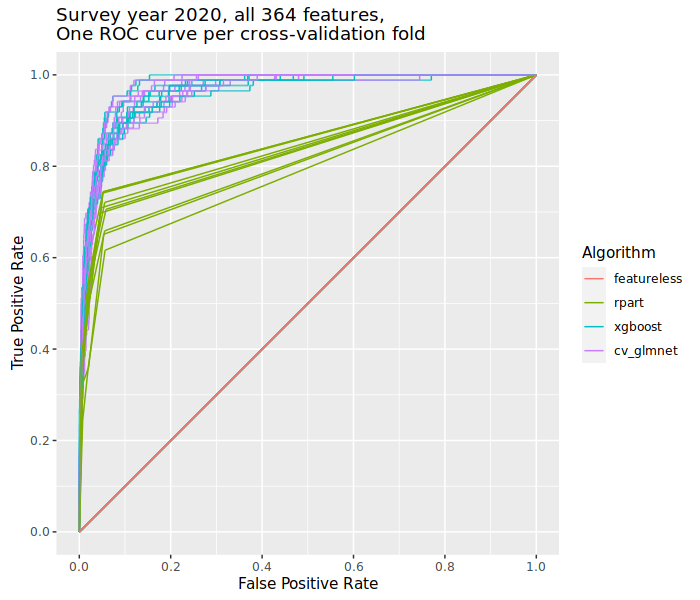
\includegraphics[width=0.9\textwidth]{download-nsch-mlr3batchmark-registry-one-set-all-features-roc.png}
\end{frame}

\begin{frame}
  \frametitle{Default prediction threshold can be viewed as a dot}
  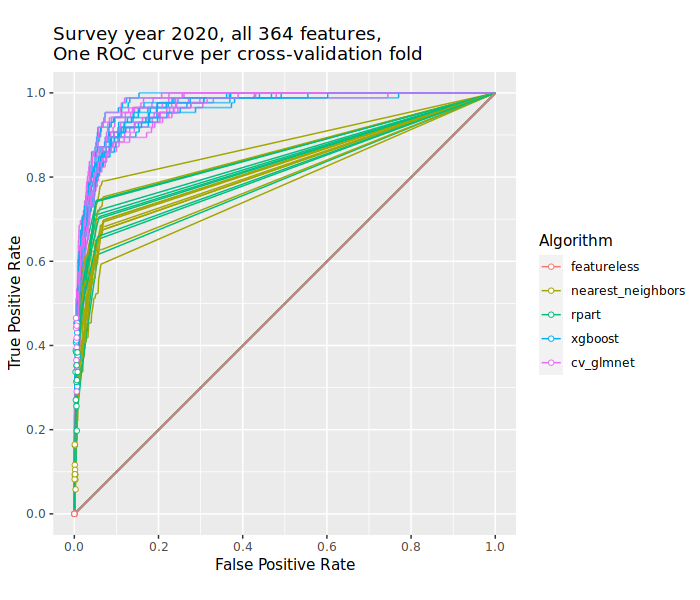
\includegraphics[width=0.9\textwidth]{download-nsch-mlr3batchmark-registry-one-set-all-features-roc-point.png}
\end{frame}

\begin{frame}
  \frametitle{Default prediction threshold can be viewed as a dot}
  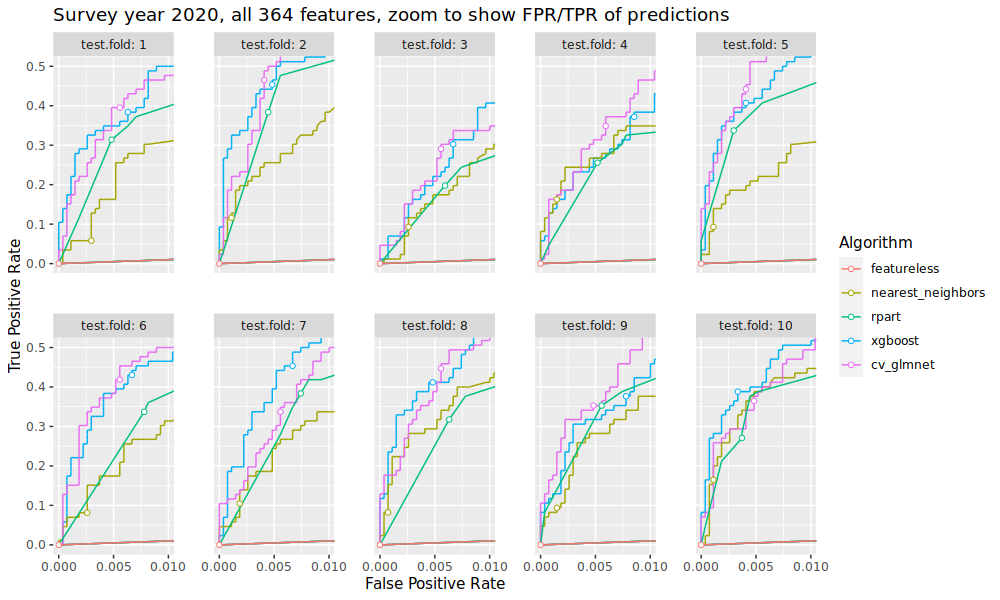
\includegraphics[width=\textwidth]{download-nsch-mlr3batchmark-registry-one-set-all-features-roc-zoom.png}

  Relatively small FPR because there are so few positive labels
  (Autism=Yes only 3\% of 27808 rows in 2020).
% > out.dt[, table(survey_year, Autism)]
%            Autism
% survey_year   Yes    No
%        2019   546 17656
%        2020   857 26951  
% > c2020=c(857, 26951)
% > c2020/sum(c2020)
% [1] 0.03081847 0.96918153
% > sum(c2020)
% [1] 27808
\end{frame}

\begin{frame}
  \frametitle{Area Under ROC Curve (AUC) quantifies accuracy over all thresholds}
  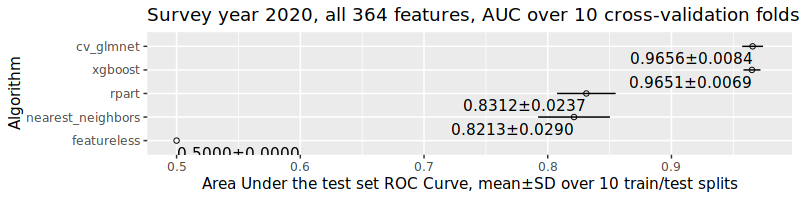
\includegraphics[width=\textwidth]{download-nsch-mlr3batchmark-registry-one-set-all-features-auc.png}
\end{frame}

\section{Model interpretation / feature selection}

\begin{frame}[fragile]
  \frametitle{Column categorization}
Each input/feature column was assigned a category.
\begin{verbatim}
column_name,category
survey_year,
Autism,
State FIPS Code=Alabama,state
...
Number of Children in Household=1,home
...
Sex of Selected Child=Male,birth
...
Deafness=Yes,comorbidity
...
               behavior       birth comorbidity 
          2          15          24          30 
    culture  healthcare        home       state 
         14          88         130          50 
     wealth 
         13 
\end{verbatim}
\end{frame}

\begin{frame}
  \frametitle{Cross-validation for category importance}
  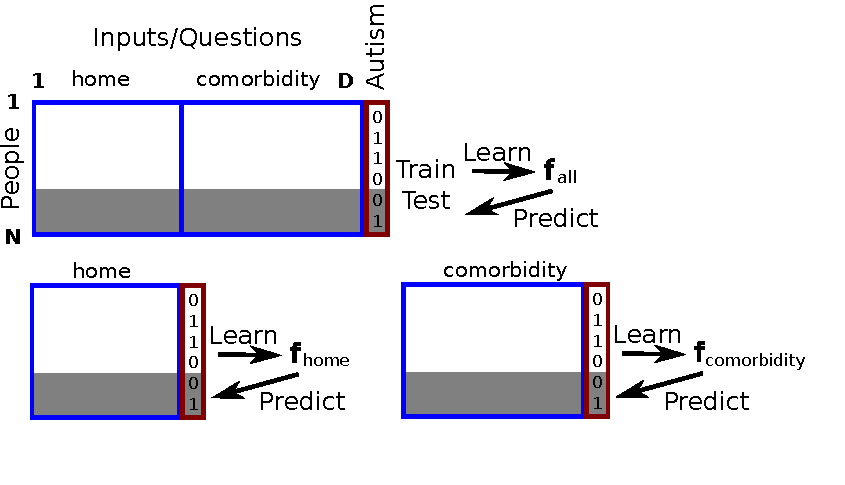
\includegraphics[width=\textwidth]{drawing-cv-feature-sets.pdf}
\end{frame}

\begin{frame}
  \frametitle{Cross-validation for category importance}
  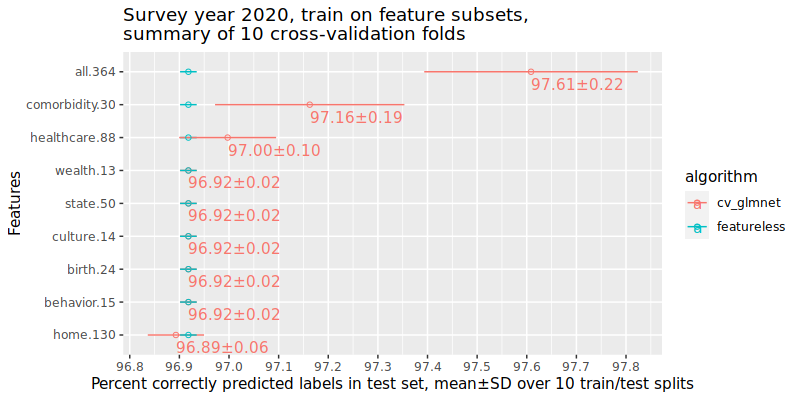
\includegraphics[width=\textwidth]{download-nsch-mlr3batchmark-registry-one-set-compare-features.png}

TODO equation

  \begin{itemize}
  \item Positive coefficients mean larger values of that feature are
    more likely to TODO
  \end{itemize}
\end{frame}

\begin{frame}
  \frametitle{Linear model coefficient / feature importance}
  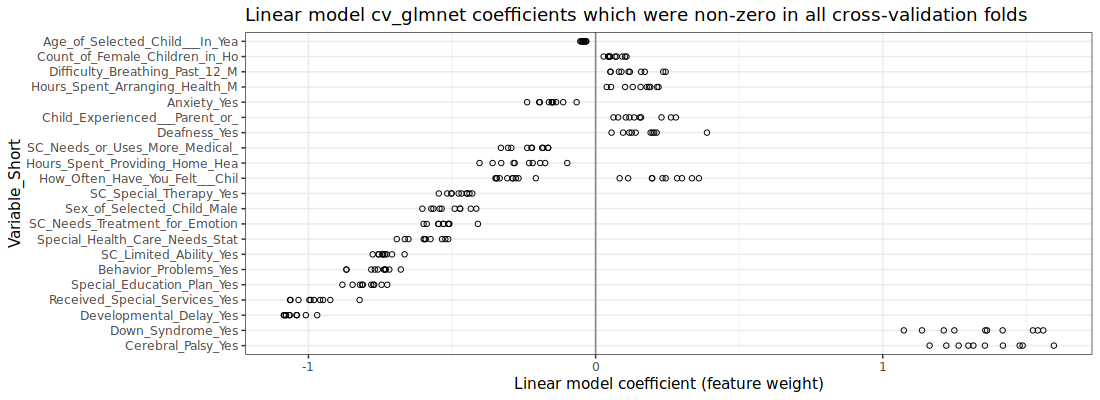
\includegraphics[width=\textwidth]{download-nsch-mlr3batchmark-registry-glmnet-coef-all.png}
\end{frame}

\begin{frame}
  \frametitle{Linear model coefficient / feature importance}
  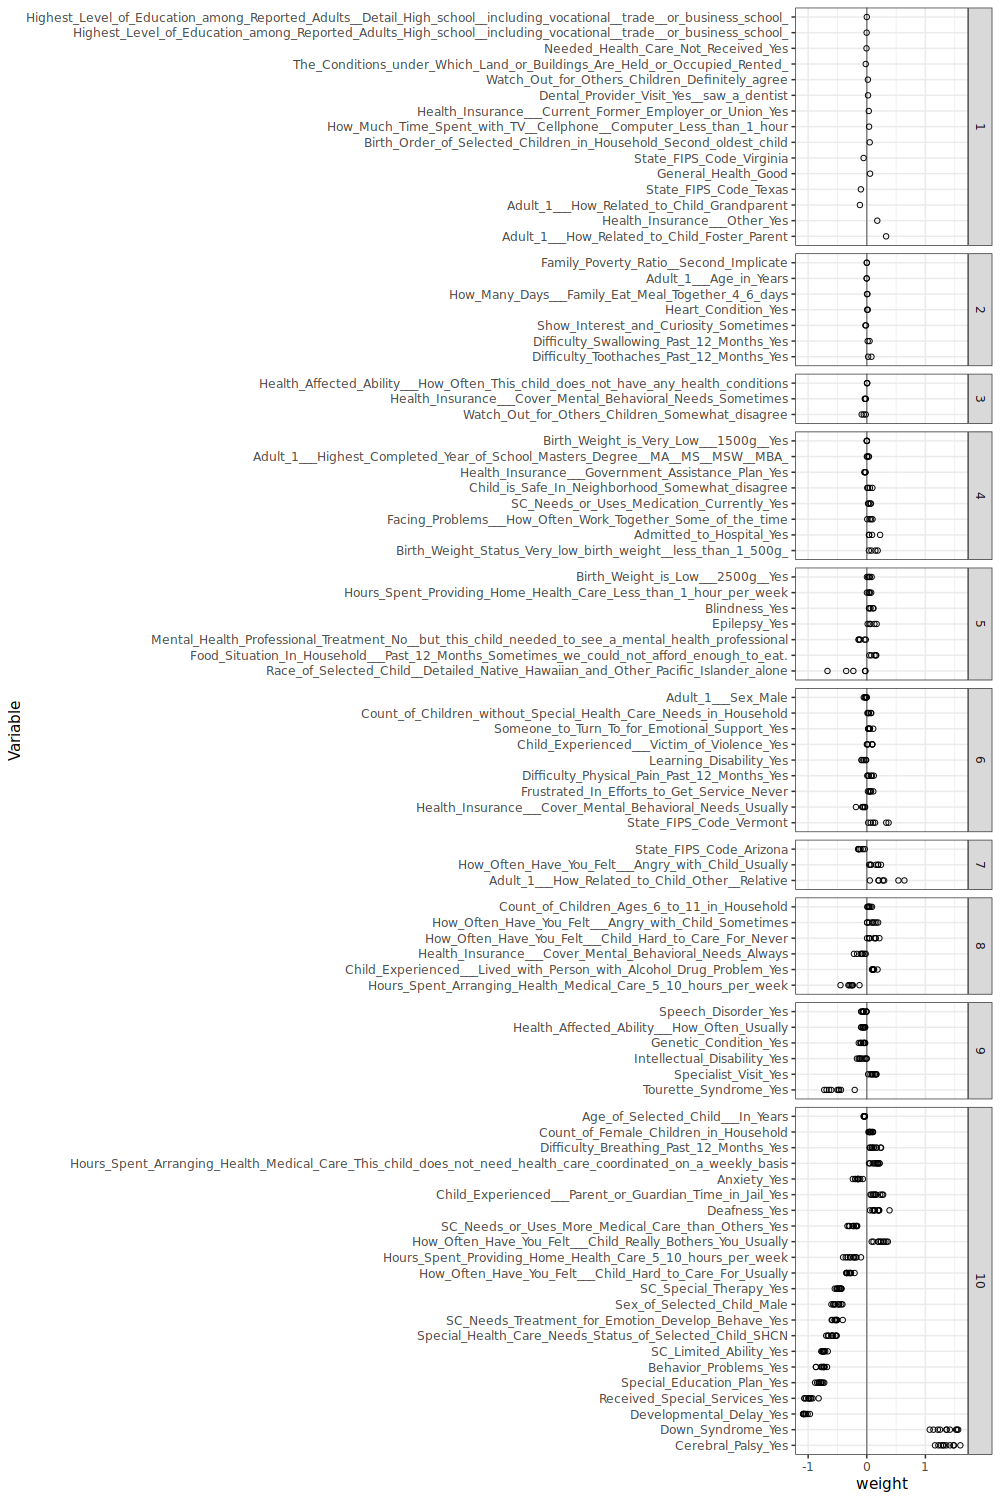
\includegraphics[height=0.7\textheight]{download-nsch-mlr3batchmark-registry-glmnet-coef.png}

  View full figure online, \url{https://github.com/tdhock/2024-01-ml-for-autism/blob/main/download-nsch-mlr3batchmark-registry-glmnet-coef.png}
\end{frame}

\section{Similarity/difference between years}

\begin{frame}
  \frametitle{Cross-validation for determining similarity between years}
  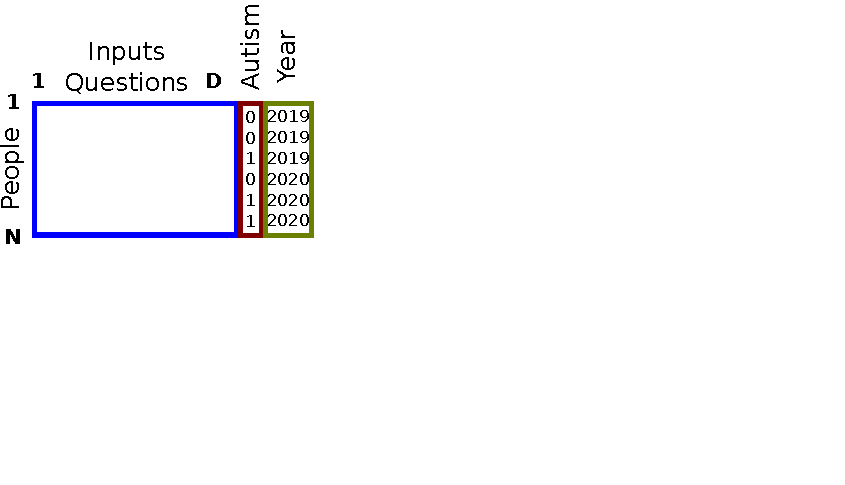
\includegraphics[width=\textwidth]{drawing-cv-same-other-years-1.pdf}
\end{frame}

\begin{frame}
  \frametitle{Cross-validation for determining similarity between years}
  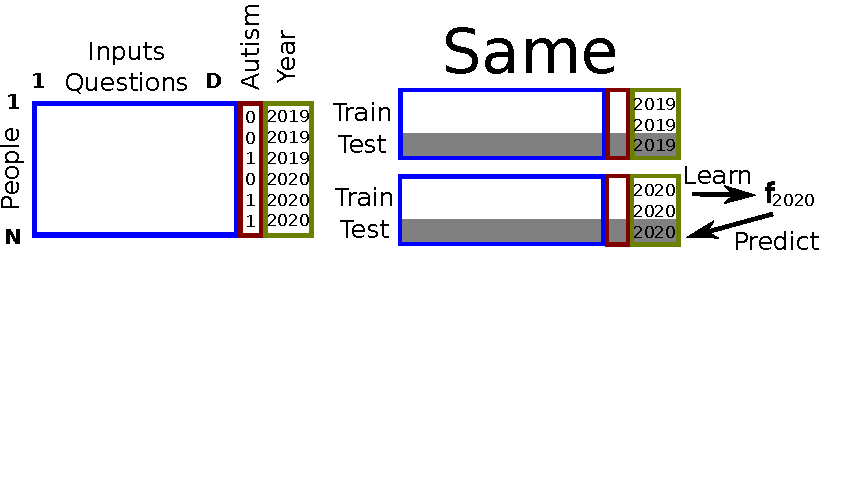
\includegraphics[width=\textwidth]{drawing-cv-same-other-years-2.pdf}
\end{frame}

\begin{frame}
  \frametitle{Cross-validation for determining similarity between years}
  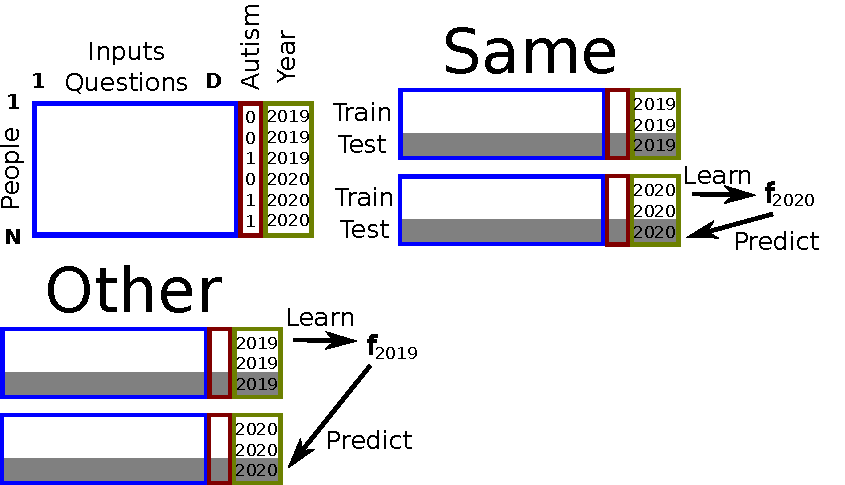
\includegraphics[width=\textwidth]{drawing-cv-same-other-years-3.pdf}
\end{frame}

\begin{frame}
  \frametitle{Cross-validation for determining similarity between years}
  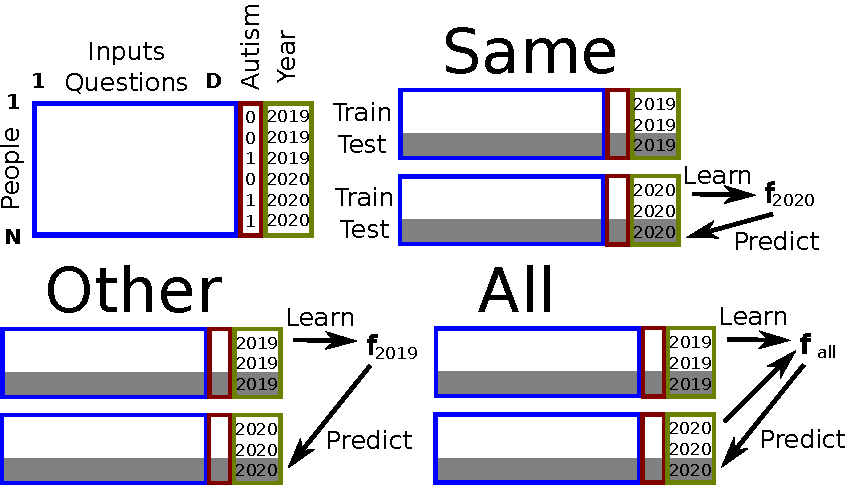
\includegraphics[width=\textwidth]{drawing-cv-same-other-years-4.pdf}
\end{frame}

\begin{frame}
  \frametitle{Cross-validation for determining similarity between years}
  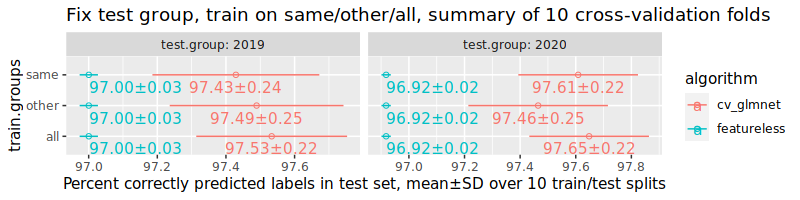
\includegraphics[width=\textwidth]{download-nsch-mlr3batchmark-registry-predict-new-year.png}
  \begin{itemize}
  \item 18,202 rows in 2019, whereas 27,808 in 2020.
  \end{itemize}
% > out.dt[, table(survey_year)]
% survey_year
%  2019  2020 
% 18202 27808 
\end{frame}

\section{Discussion and Conclusions}

\begin{frame}
  \frametitle{Discussion and Conclusions}
  \begin{itemize}
  \item Often we want to know if we have similar or different patterns
    in different groups (train on one year, predict
    on another).
  \item Cross-validation can be used to determine the extent to which
    we can train on one group, and accurately predict on another.
  \item Machine learning algorithms like L1 regularized linear models
    (LASSO/cv\_glmnet) are additionally interpretable in terms of which features
    are used for prediction (can be compared between models trained on
    different groups).
  \item Free/open-source software available: mlr3resampling R package
    on CRAN and \url{https://github.com/tdhock/mlr3resampling}
  \item Let's collaborate! Contact: toby.hocking@nau.edu,
    toby.hocking@r-project.org
  \end{itemize}
\end{frame}

\end{document}